% This file was created with tikzplotlib v0.10.1.
\definecolor{mycolor1}{rgb}{0.00000,0.44700,0.74100}%
\definecolor{mycolor2}{rgb}{0.85000,0.32500,0.09800}%
\definecolor{mycolor3}{rgb}{0.92900,0.69400,0.12500}%
\definecolor{mycolor4}{rgb}{0.49400,0.18400,0.55600}%
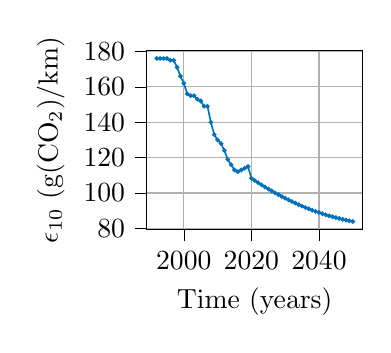
\begin{tikzpicture}

\definecolor{darkgray176}{RGB}{176,176,176}
\definecolor{steelblue31119180}{RGB}{31,119,180}

\begin{axis}[
/pgf/number format/1000 sep={},
scale = 0.4,
tick align=outside,
tick pos=left,
x grid style={darkgray176},
xlabel={Time (years)},
xmajorgrids,
xmin=1989, xmax=2052.9,
xtick style={color=black},
y grid style={darkgray176},
ylabel={$\epsilon_{10}$ (g(CO$_2$)/km)},
ymajorgrids,
ymin=79.295, ymax=180.605,
ytick style={color=black}
]
\addplot [semithick, mycolor1, mark=*, mark size=.5, mark options={solid}]
table {%
1992 176
1993 176
1994 176
1995 176
1996 175
1997 175
1998 171
1999 166
2000 162
2001 156
2002 155
2003 155
2004 153
2005 152
2006 149
2007 149
2008 140
2009 133
2010 130
2011 128
2012 124
2013 119
2014 116
2015 113
2016 112
2017 113
2018 114
2019 115
2020 108.3
2021 107
2022 105.8
2023 104.6
2024 103.4
2025 102.3
2026 101.2
2027 100.1
2028 99.1
2029 98
2030 97.1
2031 96.1
2032 95.2
2033 94.3
2034 93.4
2035 92.6
2036 91.8
2037 91.1
2038 90.3
2039 89.6
2040 89
2041 88.3
2042 87.7
2043 87.1
2044 86.6
2045 86.1
2046 85.6
2047 85.1
2048 84.7
2049 84.3
2050 83.9
};
\end{axis}

\end{tikzpicture}
